% !TEX root = Thesis.tex
\section{Offshoring in Literature}
Offshoring has been widely studied in the past decades. There are two major branches of research: the first describes reality through statistics or case studies (e.g. \cite{Rottman.2008} and \cite{Pedersen.2013}) while the second branch designs trade models to explain the discovered correlations (e.g. \cite{Antras.2004}, \cite{Grossman.2008} and \cite{Helpman.1999}).

This wealth of existing knowledge has been used for the following section, where the relevant terms of the subject are defined first. Furthermore, a brief history of offshoring is given before describing offshoring in the USA first, then offshoring in Germany.

\subsection{Definition and Terms}
In existing literature, there is no single definition of the term offshoring nor one precise delimitation to the term outsourcing. Both terms refer to sourcing decisions in companies. 

For example, according to \cite[pp. 1f]{Knolmayer.2007}, outsourcing is buying services from other companies. Offshoring is defined as a special form of outsourcing, in which the service is bought from a foreign company. On the other hand, \cite[p. 2]{Alebrand.2013} defines outsourcing and offshoring as mutually exclusive: outsourcing is the provision of services by external companies, offshoring is the internal execution of tasks in a foreign country.

These contrasting definitions may serve as an example for the lack of distinct terms in this field of research. Nevertheless all the definitions agree that outsourcing pertains to external service provision and offshoring refers to service provision in a foreign country. This Bachelor's thesis will use the following definition of the term offshoring by \cite[p. 321]{Andersson.2016}:

\begin{quote}
	``Offshoring [is the] disintegration of the firms’ production processes across national borders[...]''
\end{quote} 

This means, offshoring is not only a description for the state of an organization, but also the process to relocate business processes.

The term outsourcing is derived from ``Outside Resource Using''(\cite[p. 46]{Specht.2007b}). It is acquiring intermediate inputs from external businesses (\cite[p. 46]{Specht.2007b}).

Therefore, the terms offshoring and outsourcing do not have a direct relation; both terms are independent and describe different possibilities of entrepreneurial organization. In figure \ref{fig:DefTerms}, the delimitation between outsourcing and offshoring is clearly shown. A company can choose to offshore, outsource or both; every single possibility has its own term. Offshoring, in the context of this thesis, means foreign outsourcing and \gls{fdi}, unless otherwise specified.

\begin{figure}[htb]
	\centering
	\includegraphics[width=0.7\textwidth]{Pictures/Terms_definition}
	\caption{Definition of terms, based on \cite[pp. 552f]{Antras.2004}}
	\label{fig:DefTerms}
\end{figure}

Some publications add a geographical dimension to their definition of offshoring. \cite{Jahns.2007} state that there must be shores between the customer and the supplier in order to call the transaction offshoring, otherwise the correct term would be Nearshoring. \cite{Cappallo.2006} postulate a need for a relatively high distance ("relativ hohe räumliche Distanz", p. 487) between the partners. \cite{Dressler.2007} defines offshoring only as transaction between partners on different continents. Given the ambiguous and arbitrary nature of the distinction between offshoring and nearshoring, this thesis refrains from using the term nearshoring. All provision of services outside the captive country of a company are called offshoring.

\subsection{Factors for the Development of Offshoring}

Globalization, and offshoring as part of the development, had its early beginnings in the 1970s and gained traction once the Iron Curtain had fallen in 1989 (\cite[p. 1]{Sachs.1995}). This section describes the various factors that enabled the development of offshoring to the point it is today.

\paragraph{Political and Historical Developments}
After the end of \gls{ww2}, countries belonged to one of three distinct sectors of the world: the capitalist western countries, communist eastern companies or developing countries that sought a way to not get crushed between the two super powers and proclaimed state-led industrialization, a third way between capitalism and communism. (\cite[pp. 12f]{Sachs.1995})

With the majority of world population in countries without market-based economic mechanisms in place and most of the currencies not freely convertible, international trade was basically nonexistent in the post-war world. While western countries systematically restored their trade relations, developing countries were much slower to open their economic systems to international trade. By 1994, most countries had opened their trade policies through removing trade barriers, ensuring the free convertibility of their currencies and disestablishing state monopolies. (\cite[pp. 12-25]{Sachs.1995})

In the last twenty years, global trade relations have only increased. Trade agreements and organizations such as the \gls{wto}\footnote{For further information please see the website of WTO, \url{https://www.wto.org/}, visited on 05. \nolinebreak August 2016}, the \gls{nafta}\footnote{Further information: \url{https://ustr.gov/trade-agreements/free-trade-agreements/north-american-free-trade-agreement-nafta}, visited on 05. August 2016} or  the \gls{eec}\footnote{Established 1957 with the Treaty of Rome \url{http://eur-lex.europa.eu/legal-content/EN/TXT/?uri=URISERV:xy0023}, visited on 05. August 2016} (a predecessor of the European Union) further facilitated global trade and created a stable environment for long-term business agreements across borders. 

\paragraph{Information and Communication Technology}
Innovations in \gls{ict} have been paramount in enabling offshoring. Beginning with the invention of the first computer in 1941, the rapid development of computing power, data storage and particularly data transmission removed the need for local completion of tasks. The Internet necessitated a quick standardization and modernization of communication systems on a global scale -- the prerequisite for offshoring. (\cite[pp. 9f]{Hutzschenreuter.2007} and \cite[p. 93]{Jahns.2007})

\paragraph{Organizational Factors}
In order to efficiently offshore tasks or processes, the work has to be well-defined and standardized. In this way, economies of scale can fully be utilized and completion of work can be managed across multiple involved companies or subsidiaries. (\cite[p. 11]{Hutzschenreuter.2007})

The aforementioned developments in \gls{ict} remove the need for local presence of the service provider (Uno-Actu-Principle) for most services. Digitalization enables organizations to detach tasks from specific locations. In a first step, those tasks are centralized and standardized. The second step is often offshoring the tasks. (\cite[pp. 12f]{Hutzschenreuter.2007})
\newpage
Company size is an important indicator when describing organizational factors. Therefore, in table \ref{tab:CompanySize} a delimitation is introduced according to recommendation of European Commission\footnote{EU recommendation 2003/361: \url{http://eur-lex.europa.eu/legal-content/EN/TXT/HTML/?uri=CELEX:32003H0361&from=EN}, visited on 19. August 2016}.
\vspace{3mm}
\begin{table}[htb!]
	\centering
	\begin{tabular}{l | r c r}
		\textbf{Company category} & \textbf{Staff headcount} && \textbf{Turnover}\\ \hline
		\rule{0pt}{3ex}   Micro & $<$ \, 10 &  and & $\le$ \euro \, 2 m\\ \hline
		\rule{0pt}{3ex}   Small & $<$ \, 50 & and & $\le$ \euro 10 m\\ \hline
		\rule{0pt}{3ex}   Medium & $<$ 250 & and & $\le$ \euro 50 m\\ \hline
		\rule{0pt}{3ex}   Large & $\ge$ 250 & and & $>$ \euro 50 m\\
	\end{tabular}
	\vspace{3mm}
	%Immer caption vor label!!!
	\caption{Definition of company sizes}
	\label{tab:CompanySize}
\end{table}

\paragraph{Macroeconomic and Socio-Demographic Factors}
\Gls{ict} developments, organizational and political factors are enablers for offshoring, but the main driver for offshoring decisions in companies are the differences in salaries, taxes, and interest rates between industrialized and developing countries that result in cost arbitrage. In \cite[p. 89]{Jahns.2007}, the example of engineering wages in 2000 is given: while German and American engineers earned \$31 and \$36 per hour, an Indian engineer made only \$6.5\footnote{Figures are given with a decimal point.} per hour\footnote{The authors refer to United Nations Secretary and Industry Labor Office (2002) as source of these wages, which could not be verified at the time of writing this thesis.}. It is obvious that companies want to use this disparity to their advantage.

In addition to the wage differences, socio-demographic factors such as education, motivation and age distribution in developing countries influence offshoring supply. High social prestige connected to working for large western companies contributes to a higher ratio of academics that apply for offshoring related jobs and motivates employees. Thus, the quality of work is often very good and may be better than in the original country. (\cite[p. 93]{Jahns.2007})

In the following sections, those factors for both the USA and Germany will be examined. Furthermore, a quantification of offshoring will be attempted in order to provide a basis for the direct comparison of both countries in section \ref{sec:DifferencesUSGER}.

\subsection{Offshoring in the USA}
\label{sec:OffshoringUS}

\begin{quote}
	``The United States is the world's largest direct investor[...]'' \linebreak(\cite[p. 3]{Kozlow.2006})
\end{quote}

Offshoring originated in the USA and spread from there as a trend around the globe. This section explores the contributing factors from historical, organizational and macroeconomic angles. It is then completed by a quantitative evaluation of offshoring in the USA.

\paragraph{Political and Historical Developments} \label{par:USHistory}
The United States, with its country intact and victorious in \gls{ww2}, emerged as one of two global super powers in the post-war world. On an economical level, the U.S. quickly confirmed its position as the world's richest country. Between 1940 and 1960, gross national product more than doubled from \$200 \nolinebreak bn to \$500 \nolinebreak bn. In the same time, large American corporations grew even larger in a wave of mergers, resulting in conglomerates with operations in a variety of industries. In this time, the first companies developed holdings overseas and, in that way, pioneered the development of offshoring. (\cite{Winkler.1994b})

As confrontations between the Soviet bloc and the U.S. slowly escalated to the Cold War in the 1960s, the American government ran unprecedented research and innovation programs. Military-funded inventions such as \acrshort{arpanet} lay the groundwork for the development of the Internet (\cite{Leiner.2003}), while the race to space culminated in the first man on the moon in 1969. Surrogate wars, most notably Vietnam War, strained the national economy\footnote{This section is focused on the economical circumstances that contributed to the development of offshoring. Therefore, social and societal effects of Vietnam War are not included for the sake of a stringent argumentation.}, so that by the start of the 1970, the country was in a deep recession. The Dow Jones Index fell 36 percent between November 1968 and May 1970; in the same time, unemployment rates reached 6.6 \%, and by 1973 inflation rose to 9 \%. President Carter, elected in 1976, tried to turn the economy around by means of government spending and deregulation.
(\cite{Winkler.1994})


In the 1980s, a trend that had started 50 years ago culminated in three-fourths of all employees working in the service sector. This trend has been facilitated and accelerated by availability and use of computers, a technology the U.S. government had made significant investments in since the 1950s. At the same time, classic industries such as automobile, steel and textile were suffering from increased competition. Combined with falling oil prices in 1982, a sharp recession had more than 10\% of the population unemployed. President Reagan reacted with tax cuts and by 1984 the economy had turned around and entered a five-year period of growth.
(\cite{Winkler.1994c})

Relations between the superpowers began to normalize in the late 1980s. All over Eastern Europe, people were demonstrating for democratic reforms. In 1989, the Berlin Wall fell. With the end of the Cold War, the wold was open once again, open for global trade.
(\cite{Winkler.1994c})

To recap, the most important phenomena in recent U.S. history with respect to offshoring are:
\begin{itemize}
	\item Quick economic recovery after \gls{ww2}
	\item The expansion of large, multi-industrial corporations
	\item Government investment in research, yielding the basis for offshoring enabling technology
	\item The tendency to react with increased spending to economic downturns
	\item Economic deregulation in the late 1970s
	\item Growing importance of the service sector
	\end{itemize}
In 1993, U.S. congress approved \acrlong{nafta}, the first free trade agreement of its kind, after a heated national debate. Labor unions insisted that \acrshort{nafta} would lead to job losses, environmentalists worried that it would encourage companies to bypass controls on industrial pollution, and government argued, a greater exchange of goods and services would make the three participating countries\footnote{USA, Mexico and Canada} more competitive in global markets(\cite{Winkler.1994c}). With this, the era of offshoring began.

\paragraph{Organizational Factors}
When analyzing organizational structure of U.S. economy, there is no way around the United States Census Bureau. Every five years, the authority conducts a Survey of Business Owners and Self-Employed Persons. The most recent installment selected 1.75 million businesses in 2012 asking for information regarding characteristics of the businesses and their owners. Data was then matched to existing information from the Internal Revenue Service and further census data\footnote{For a complete description of census methodology please refer to \url{http://www.census.gov/programs-surveys/sbo/technical-documentation/methodology/2012-sbo-methodology.html}, visited on 20. August 2016}.

\bildcite{US_Company_Size}{Size of U.S. companies by number of employees}{fig:USCompSize}{Data source: \url{http://factfinder.census.gov/faces/tableservices/jsf/pages/productview.xhtml?pid=SBO_2012_00CSCB42&prodType=table}, visited on 19. August 2016}{0.5}

In figure \ref{fig:USCompSize} the number of companies per size category is plotted on a pie chart. Remarkably, micro companies make up about  three-fourths of all companies. Another fifth are small companies. As the U.S. Census Bureau uses a different scale to classify company sizes than presented in table \ref{tab:CompanySize}, a delimitation between medium and large companies is not possible, but the low number of companies with more than 500 employees (17 724, or 0.33\%) is noteworthy.

Before any conclusions are made, a different angle of analysis is added in order to gain a comprehensive view on U.S. economy. 

\bildcite{US_Employees}{Number of employees per company size in the U.S.}{fig:USEmployees}{Data source: \url{http://factfinder.census.gov/faces/tableservices/jsf/pages/productview.xhtml?pid=SBO_2012_00CSCB42&prodType=table}, visited on 19. August 2016}{0.5}

In figure \ref{fig:USEmployees}, the number of employees working in companies of each size categories is shown. The outstanding fact is that 53\% of the working American population, 60 \nolinebreak825 \nolinebreak680 persons, are employed at the 17 \nolinebreak724 companies with more than 500 employees. On the other hand, micro companies only employ 10\% of working population.

This means that large companies have a significant influence on U.S. economy. As mentioned on page \pageref{par:USHistory}, in U.S. history there have been several waves of mergers that resulted in large, multi-industry companies (\cite{Winkler.1994b}). In consequence, many corporations that dominate global markets today are American (e.g. The Coca Cola Company, Procter \nolinebreak \& \nolinebreak Gamble, General Electric). 


\paragraph{Macroeconomic and Socio-demographic Factors}
The USA spans 9 984 670 square kilometers and five time zones\footnote{Considering no overseas terrorities.}. This makes the country the third largest in the world by area. (\cite{CentralIntelligenceAgency.2016})

Therefore, U.S. citizens are already used to dealing with large distances and different time zones, maybe from working in a company that operates nationwide, maybe because friends or family live in different states. Cross-country relocations are fairly common, and TV air times are always given in the different time zones for the convenience of the viewers. Offshoring profits from this circumstance, because even though the distance to co-workers increases, the communication behaviors needed for collaboration across a distance are already in place.



%College system


\paragraph{Offshoring Quantified}
Offshoring originated in the USA in the early 1990s (\cite[p. 389]{Pisani.2016}). Even earlier, U.S. companies pioneered in foreign investment, e.g. by establishing production sites abroad (\cite[p. 5]{Kozlow.2006}). Looking at the past 25 years, imports of services and especially imports of \gls{ict} services have grown exponentially. In figure \ref{fig:US_ICT_Import}], import volume for \gls{ict} services is shown. Short of a small decline in 2002, which can be explained with the burst of the Dotcom Bubble in the same year, volumes have consistently grown and tripled from \$12 bn in 1999 to \$36 bn in 2015. Since 2010, the growth has slowed down considerably. It remains to be seen if this trend persists or if it is just a small break that will make way to further growth.

\bildcite{US_Import_ICT_Services}{U.S. import of \glsentryshort{ict} services}{fig:US_ICT_Import}{Data source: \url{www.bea.gov/newsreleases/international/trade/trad_time_series.xls}, visited on 10. August 2016}{0.6}

A comprehensive look at the prevalence of offshoring in the U.S. can be gained by consulting the Survey of Business Owners and Self-Employed persons. An overview of relevant findings is given in figure \ref{fig:USOffshoringPercent}.

In this graph, for each company size there are several percentages given. First, the percent of firms that size which outsourced or transferred any business fuction or service to a company outside the U.S. is shown. Predictably, all but the biggest company size with more than 500 employees have a low share of companies that practice foreign outsourcing. However, even of the biggest companies, only 7.1 \% have used this method of offshoring in 2012.

Additionally, there are the percentages of revenue and number of employees of companies which outsourced outside of the U.S. in 2012 shown. In most size categories, companies have a bigger share of revenue than what would be suggested by their number. This leads to the conclusion that companies that outsource abroad earn more revenue than those who don't.

\bildcite{US_Offshoring_percentage}{Results of 2012 Survey of Business Owners - U.S. Census Bureau}{fig:USOffshoringPercent}{Data source: \url{http://factfinder.census.gov/faces/tableservices/jsf/pages/productview.xhtml?pid=SBO_2012_00CSCB42&prodType=table}, visited on 19. August 2016}{0.9}

Data regarding foreign direct investments of U.S. companies in context of offshoring is not as readily available; in fact, ``[...]no U.S. government agency collects data on U.S. firms in such a way that it is possible to track a plant closing in the United States with a comparable plant opening in a foreign country. As a result, most data on the activity of U.S. firms shifting plants or jobs abroad are anecdotal.'' (\cite{Jackson.2013})


Often, one company may outsource to a different company in the U.S., which in turn could use a subcontractor in a different country. In this scenario, no company has actively shifted jobs abroad, but there is still an impact on the employment market. An estimation by \gls{bea} of job losses due to offshoring was 195 \nolinebreak000 jobs per year from 1999 to 2001, which is only 1.5\% of the 13 million jobs that were lost overall per year. (\cite[pp. 14ff]{Kozlow.2006})

It is expected that the share of U.S. companies which offshore through \gls{fdi} is much higher than the 7.1\% of large companies that use foreign outsourcing. In \cite[pp. 167ff]{Hutzschenreuter.2007}, a study of 231 American companies is presented. Of those, 60\% have implemented offshoring. Considering the small sample size and the fact that only large companies have been invited to participate in the study (\cite[pp. 199f]{Hutzschenreuter.2007}) it can be assumed that this number is much lower. Unfortunately, research did not uncover a more precise estimation.

\subsection{Offshoring in Germany}
\label{sec:OffshoringGER}
In this section, the main factors determining offshoring ventures of German companies will be explored, starting with a short excursion in recent history, then discussing organizational and macroeconomic and socio-demographic factors. At last, the scale of offshoring in Germany is quantified.

\paragraph{Political and Historical Developments}
In the aftermath of \gls{ww2}, German economy was devastated. Vast areas of the country were destroyed by allied bombs, including cities and production plants. The country was divided into four military occupation zones, one of which would become the soviet-influenced \gls{ddr} in 1949. (\cite{BBC.2012})

In \gls{ddr}, the Soviet Union undertook an extensive industrial dismantling, while similar plans had not been executed in the allied occupation zones, which in 1949 formed the \gls{brd}. Still, reconstruction of West German economy progressed very slowly. Facing the threat of communist ideology spreading in Europe, U.S. Secretary of State Marshall established the ``Marshall Plan'', which allowed participating countries to receive U.S. goods and raw materials while paying in their local currency. This was the foundation for a rapid growth of West German economy between 1950 and 1960, the so-called `Wirtschaftswunder'. (\cite{Kimmel.2005})

The same time frame saw a deepening of the division of the country. While \gls{ddr} joined the soviet Warsaw Pact in 1955, West Germany joined the \gls{nato} in the same year and the \gls{eec} in 1957. This development culminated 1961 in the construction of the Berlin Wall. (\cite{BBC.2012})

From an economic perspective, \gls{brd} had quickly become a valued trading partner and important exporter of industrial machine tools, automobiles, and chemical and engineering products to the western hemisphere. In spite of suffering from restrictions of the communist regime, \gls{ddr} assumed a similar role in the communist part of the world, exporting machine tools, electronics and chemicals. The 1960s brought firsts signs of economic slowdown, in part due to the stop of intra-German migration from east to west that had supplied the west with skilled labor until 1961. Under the pressure of consolidation in the late 1960s, the new Grand Coalition in \gls{brd} increased regulation of the economy.
(\cite{Solsten.1995}\footnote{This book was accessed online, therefore page numbers can not be given. The cited information  is found in chapters ``The Economy'' and ``The Economic Miracle and Beyond'', \url{http://countrystudies.us/germany/134.htm} and \url{http://countrystudies.us/germany/137.htm}, visited on 22. August 2016})

By the 1980s, the intra-German diplomatic relationship hat normalized to a point where it was possible for West Germans to visit the \gls{ddr}. Soviet president Mikhail Gorbachev started reforms  mid-decade in order to liberalize the Soviet Union and stabilize the economy. Even though these reforms were disapproved of by East German government, the news reached people in the \gls{ddr} and encouraged opposition. In spite of facing rising repression by the government, opposition groups grew large enough to organize large public demonstrations in 1989. Additionally, many \gls{ddr} citizens fled the country through neighbor states, particularly Hungary. East German government caved to the pressure and opened the Berlin Wall on 9. November 1989. The following year, West German Chancellor Kohl and the first freely elected \gls{ddr} government created the legalistic and diplomatic prerequisites for reunification. On 3. October 1990, Germany was reunited.
(\cite{Solsten.1995}\footnote{Chapter ``History: 1945 to 1990, \url{http://countrystudies.us/germany/3.htm}, visited on 23. August 2016})

As the Cold War had ended, the path for even stronger European integration was clear. In 1992, twelve European nations signed the Treaty of Maastricht on European Union\footnote{Further information can be found at EUR-Lex: \url{http://eur-lex.europa.eu/legal-content/EN/TXT/?uri=uriserv:xy0026}}, creating the European Union and prepared the introduction of a common currency with financial criteria that are to be met by each member in order to adopt the currency. The euro was introduced as an accounting currency in 1999 and in 2002 the original members of the Eurozone replaced their national currencies with euros.
%Euro

Summing up, the most important historical developments for offshoring in Germany are:
\begin{itemize}
	\item Strong focus on exports
	\item \textit{Wirtschaftswunder} in the 1950s
	\item Goverment regulation of economy
	\item Founding member of the EU
	\item Euro as common currency in the EU
\end{itemize}

\newpage %CHECK

\paragraph{Organizational Factors}
Germany's economy is largely influenced by \gls{sme}. Many companies have found their niche where they excel and dominate the market. Often, those companies are family-owned, managed by the owner(s) and rooted in their local community. These qualitative characteristics are not useful for statistical analysis, therefore, \gls{sme} are defined by number of employees and revenue as shown in table \ref{tab:CompanySize}.

\begin{figure}[htb]
	\centering
	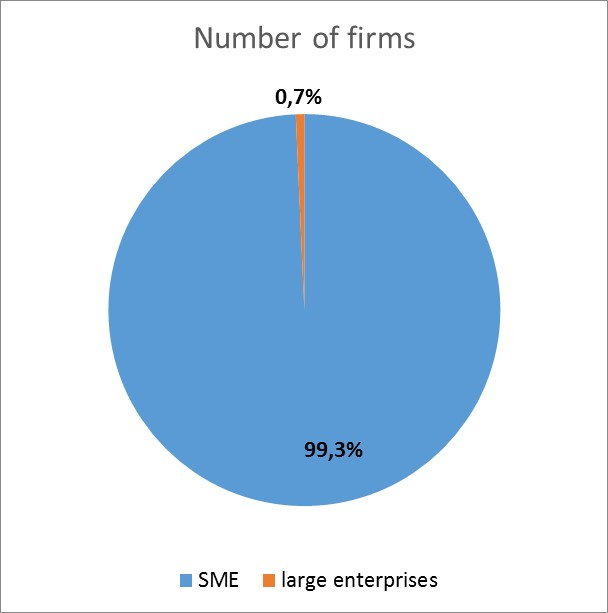
\includegraphics[width=0.4\textwidth]{Pictures/GER_Company_Size}
	\caption{Percentage of \acrshort{sme} and large companies in Germany, 2011 (\cite[p. 42]{Sollner.2014})}
	\label{fig:GERCompSize}
\end{figure}

\begin{figure}[htb]
	\centering
	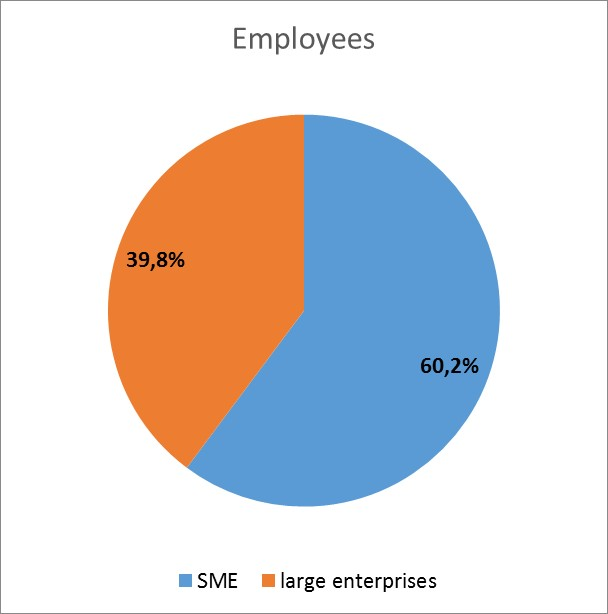
\includegraphics[width=0.4\textwidth]{Pictures/GER_Employees}
	\caption{Percentage of employees in \acrshort{sme} and large companies in Germany, 2011 (\cite[p. 42]{Sollner.2014})}
	\label{fig:GEREmployees}
\end{figure}

In figures \ref{fig:GERCompSize} and \ref{fig:GEREmployees}, percentages of \gls{sme}, large enterprises and their employees in 2011 are shown. The majority of German working population work in \gls{sme}, so those are often seen as very important for growth and structure of German economy (\cite[p. 40]{Sollner.2014}). Conversely, large enterprises are just 0.7\% of all companies, but they earn 66.5\% of revenues (\cite[p. 42]{Sollner.2014}). Those companies are more likely to engage in offshoring, because economies of scale promise larger cost savings.

Historically, Labor Unions are very strong in Germany. Despite the fact that offshoring often does not have a fundamental impact on employment in the original country, Unions often oppose offshoring plans and present a major obstacle to German companies who wish to offshore. Lengthy negotiations make it impossible for managers to move quickly and the result often hampers possible cost savings.

Both of those unique factors deter many German companies from offshoring, even though cost pressure has increased over the last two decades.

\paragraph{Macroeconomic and Socio-demographic Factors}
There are two\footnote{In the last two decades, dual degree and vocational training programs have gained traction. Offering both an academic degree and working experience, those programs are very popular and have even been implemented in American subsidiaries of German companies, e.g. Volkswagen.} basic systems of education in Germany. One is pursuing an academic degree, the other is vocational training in combination with adapted school that caters to the respective job description. This system ensures well-trained employees in both academic and non-academic jobs and is unique to Germany and Austria. As a result, employers can assume a certain level of domain knowledge in new employees. This results in shorter training times for new employees. On the other hand, knowledge transfer is often informal and not standardized or documented. Employees tend to hold their position for long times, building specialized knowledge in their working fields. 

Germany, being a small and densely-populated country, is very conductive to local collaboration. \Gls{sme} especially are very focused on their main location and even in larger companies, employees tend to build location-specific networks. When facing a problem, the first approach to solve it involves finding and speaking to someone who had this problem before. This approach often is very successful, as fluctuation in more senior employees is low and the aforementioned specialized knowledge that is built up over the course of a career at a company. Also, there may be no alternative to relying on co-workers, because this kind of intrinsic knowledge remains often undocumented.


\paragraph{Offshoring Quantified}
According to \cite[p. 70]{Eickelpasch.2015}, only 9.3 \% of business services have been imported in 2010\footnote{The author cites input-output tables of  Statistisches Bundesamt and calculations of DIW Berlin.}. This may seem like a very low number, even though it is expected that fewer German companies offshore, compared to the USA. However, Eickelpasch only accounts for Foreign Outsourcing as his definition of offshoring does not include \glspl{fdi}(\cite[p. 56]{Eickelpasch.2015}). This information is therefore not sufficient to draw any conclusions concerning offshoring in Germany.

Further insights into the prevalence of offshoring in Germany can be found in a survey that has been conducted by German Statistisches Bundesamt in 2008. For this survey, 9361 manufacturing and service companies answered a questionnaire focusing on drivers, scope and results of offshoring on firm-level (\cite[p. 7]{StatistischesBundesamt.2008}). Of the polled service companies\footnote{The survey is on shifting business activities abroad, so it includes production abroad. This thesis focuses on offshoring services, so only results of service companies are included.}, 15.4\% had offshored one or multiple corporate functions until 2006, and 10.7\% planned to do so in the time span 2007 - 2009. The percentage of companies that offshore grows with the number of employees. (\cite[p. 11]{StatistischesBundesamt.2008})

Regarding cooperation partners, the survey found that 81.4\% of service companies practiced or planned \gls{fdi} and only 24.7\% chose Foreign Outsourcing, transferring tasks to external partners. Most often, a new subsidiary had been established (47.5\%). (\cite[p. 18]{StatistischesBundesamt.2008})



\subsection{Significant Differences between Germany and the USA}
\label{sec:DifferencesUSGER}
As shown in the previous sections, there are vast differences between Germany and the USA when it comes to offshoring. However, accurately quantifying those differences is no small effort. Government institutions for measuring trade activities exist in both countries, but there are no international standards regarding the indicators. Furthermore, both economies vary largely in size. The U.S. are the worlds largest economy with a \gls{gdp} of \$17.947 trillion in 2015, while Germany had a \gls{gdp} of \$3.356 trillion\footnote{Data source: World Bank, \url{http://data.worldbank.org/indicator/NY.GDP.MKTP.CD?locations=US-DE&start=1990}, visited on 14. August 2016}. Therefore, one can not simply compare unadjusted offshoring volume.

\paragraph{Economic Focus}
As detailed in section \ref{sec:OffshoringGER}, Germany has been an export-oriented country since the 1950s. In fact, German authorities have registered trade surpluses since 1952 without exception (\cite{StatistischesBundesamt.2016}).
In contrast, the U.S. have registered consistent trade deficits in the last 30 years\footnote{Data source: U.S. Census Bureau, Foreign Trade: \url{https://www.census.gov/foreign-trade/balance/c0015.html}}. This suggests that the U.S. has an import-oriented economy. 

This discrepancy, on the first glance, does not imply anything about offshoring. On nearer inspection, though, there are two aspects. First, offshoring, as far as foreign outsourcing is concerned, is part of the foreign trade balance. Second, exporting and importing are two different mindsets that manifest in companies. For an import-oriented company, importing business services suggests itself, whereas for an exporting company this idea is not nearly as obvious.

\paragraph{Maturity of Offshoring}
American companies have a long history of collaboration with foreign countries, be it own subsidiaries (\gls{fdi}) or foreign outsourcing. The first foreign subsidiaries have been founded by U.S. companies in the 1950s (see page \pageref{par:USHistory} for details). German companies, being located in a less stable environment during Cold War, were overall less expansive and generally started to internationalize in the 1990s.

\paragraph{Structure of organizations}
Even though the quantitative distribution of companies in size categories in Germany and the U.S. is similar, there is a vast difference in the influence the different categories have on national economies. In Germany, \gls{sme} employ 60\% of the work force and earn 33.5 \% of revenues (\cite{Sollner.2014}), whereas in the U.S., large corporations with more than 500 employees\footnote{Please note that the American category system is not matchable to the European categories that are used in this thesis. U.S. Census Bureau differentiates companies from 100 to 499 employees from companies with more than 500 companies, whereas large companies in the European definition have more than 250 employees.} employ 53\% of the working population and earn 65\% of revenue\footnote{{Data source: \url{http://factfinder.census.gov/faces/tableservices/jsf/pages/productview.xhtml?pid=SBO_2012_00CSCB42&prodType=table}, visited on 19. August 2016}}.


\paragraph{Offshoring Locations and Distances}
%94\% of American Offshoring Destinations: ``Farshore'', Germany: 52 Near, 48 Farshore \cite[pp. 175f]{Hutzschenreuter.2007}
\cite{Hutzschenreuter.2007} compare their own study of 178 German companies to a similar study of 447 American companies regarding the offshoring locations that are preferred by each country. For German companies, European countries have with 52\% a slight majority over farshore\footnote{The authors define farshore-offshoring as offshoring on a different continent.} regions such as India or Brazil. (\cite[p. 175]{Hutzschenreuter.2007})

American companies however largely prefer farshore countries for their offshoring endeavors. 94\% of offshoring activities are relocated to a different continent, specifically 67\% in Asian countries. Of those 67\%, 41\% are offshoring activities in India. (\cite[p. 175]{Hutzschenreuter.2007})


\paragraph{Language} English is a language that is spoken all over the world. With 400 million native speakers it is one of the largest languages of the world, but as the \textit{lingua franca} of global business and with over 1.5 billion speakers all over the world (\cite[p. 1]{Hogg.2008}), companies operating in English have a great advantage when communicating with offshore service providers.

In comparison, German is spoken by about 100 million native speakers and in 2015, had been learned by 15.4 million people around the globe (\cite{AuswartigesAmt.2015}). This severely limits the pool of viable service providers, if German companies require the provision of services in German.
